% Numbers come from artifacts/reported_results/2026-09-30-reward-service/ (see its README).
% Generated by artifacts/reported_results/2026-09-30-reward-service/generate.py; do not edit.
\newcommand{\RSLocalBackends}{19}
\newcommand{\RSServiceScorers}{13}
\newcommand{\RSGenEstimate}{73}
\newcommand{\RSSmallBase}{102.0}
\newcommand{\RSSmallSerial}{86.9}
\newcommand{\RSSmallOverlap}{82.3}
\newcommand{\RSSmallSerialSaving}{14.8\%}
\newcommand{\RSSmallOverlapSaving}{19.4\%}
\newcommand{\RSSmallOverlapWindow}{54.8}
\newcommand{\RSLargeBase}{155.0}
\newcommand{\RSLargeSerial}{138.8}
\newcommand{\RSLargeOverlap}{140.1}
\newcommand{\RSLargeSerialSaving}{10.4\%}
\newcommand{\RSLargeSerialMin}{138.2}
\newcommand{\RSLargeSerialMax}{139.8}
\newcommand{\RSLargeOverlapMin}{138.1}
\newcommand{\RSLargeOverlapMax}{142.9}
\newcommand{\RSLargeWindow}{54.7}
\newcommand{\RSSmallWholeService}{3.08}
\newcommand{\RSSmallMicroService}{1.20}
\newcommand{\RSSmallWholeWork}{24.6}
\newcommand{\RSSmallMicroWork}{38.5}
\newcommand{\RSSmallWholeWaitMax}{24.6}
\newcommand{\RSSmallSerialFirstWaitMax}{9.6}
\newcommand{\RSSmallSerialLaterWait}{1.3}
\newcommand{\RSSmallOverlapWork}{37.7}
\newcommand{\RSLargeWholeService}{9.61}
\newcommand{\RSLargeWholeWork}{76.9}
\newcommand{\RSLargeFirstArrival}{18.2}
\newcommand{\RSLargeSerialService}{3.76}
\newcommand{\RSLargeSerialWork}{120.4}
\newcommand{\RSLargeSerialWorkMin}{119.7}
\newcommand{\RSLargeSerialWorkMax}{121.4}
\newcommand{\RSLargeOverlapWork}{121.8}
\newcommand{\RSLargeOverlapWorkMin}{119.5}
\newcommand{\RSLargeOverlapWorkMax}{124.5}
\newcommand{\RSLocalBase}{56.0}
\newcommand{\RSLocalSerial}{52.4}
\newcommand{\RSSmallShallowBase}{52.2}
\newcommand{\RSSmallShallowSplit}{57.2}
\newcommand{\RSLargeShallowBase}{86.1}
\newcommand{\RSLargeShallowSplit}{100.7}
\newcommand{\RSTrainRemoteNoCollect}{192.2}
\newcommand{\RSTrainRemoteCollect}{178.1}
\newcommand{\RSTrainLocalNoCollect}{58.0}
\newcommand{\RSTrainLocalCollect}{54.5}
\newcommand{\RSLargeWholePerPair}{0.30}
\newcommand{\RSLargeMicroPerPair}{0.47}
\newcommand{\RSSmallWholePerPair}{0.096}
\newcommand{\RSSmallMicroPerPair}{0.150}
\newcommand{\RSMpsThreeLight}{24.9\%}
\newcommand{\RSMpsTwoLight}{9.6\%}


\section{Case Study I: Reward Serving and Generation--Reward Overlap}
\label{sec:reward}

Reward evaluation is the one role in the feedback loop whose computational cost is independent of the policy architecture.
A lightweight contrastive preference model scores a batch in well under a second, whereas a vision--language judge with tens of billions of parameters can take as long as the generation it evaluates, requires a separate software environment from the trainer, and may not fit alongside the policy on the same accelerator.
UniRL therefore fixes the reward interface at the trajectory boundary while treating placement, environment isolation, and scheduling relative to generation as orthogonal execution choices.

\paragraph{Source scope.}
This case study examines UniRL commit \texttt{651490e} (2026-09-30), which postdates the v0.2.0 design-audit commit analyzed in Sections~\ref{sec:trajectory}--\ref{sec:instantiations}, together with the shared-GPU mechanism proposed in UniRL pull request~\#492 (commit \texttt{8bb4119}).
The measurements in Section~\ref{sec:reward-results} were collected as a standalone systems case study outside the E0--E6 evaluation program; their per-rollout records and table generators are archived in \codepath{artifacts/reported\_results/2026-09-30-reward-service/}.

\subsection{Scoring Contract and Failure Semantics}
\label{sec:reward-contract}

A trainer invokes a single method, \texttt{score\_and\_attach}, on the reward role.
The call is scattered across tree-complete shards like any other distributed role method (Section~\ref{sec:execution}); on each shard it constructs a typed request from the trajectory, queries a configured backend for scores, and returns an updated trajectory whose frontier layer carries a scalar reward and named component rewards per row.
The request contains the frontier layer's decoded values, non-text values from earlier turns as conditioning (for example, the source image in an image-editing task), both the original root prompt and the rewritten generation prompt, and the sample and group identifiers.
Each backend specifies which prompt field it scores against; when a prompt-rewrite stage precedes generation, the two prompts differ, and this configuration determines whether the reward measures fidelity to the original user request or to the rewritten prompt.

To prevent silent propagation of invalid credit, the reward role enforces strict validation on scored outputs.
It rejects a frontier layer that already carries rewards, raises an exception when any row fails rather than substituting a default zero (remote backends treat any non-finite score as a failure), and assigns zero reward or a configured length penalty to free-length autoregressive traces that hit the token limit without terminating.
For audio--video generation, it also rejects training reward configurations that assign zero weight to prompt-to-video alignment, because optimizing an audio--video agreement score alone permits degenerate solutions that collapse both streams; such scores remain permitted in evaluation-only mode.
Because group-normalized advantage estimation couples every sibling under a prompt, a single corrupted reward would contaminate the entire group; failing closed prevents corrupted updates from entering the optimizer.

Table~\ref{tab:reward-scorers} summarizes the scorers that implement this contract: \RSLocalBackends{} in-process backends and \RSServiceScorers{} scorers available in the standalone reward service's registry.
These span contrastive and preference models such as CLIP, PickScore, HPS, and ImageReward~\citep{radford2021clip,kirstain2023pickapic,wu2023hpsv2,ma2025hpsv3,xu2023imagereward}, vision--language judges for composition, rendered text, and instruction-guided editing~\citep{kamath2025geneval2,wu2025editreward,luo2025editscore}, video and audio--video alignment models, and text verifiers for reasoning tasks.
A remote backend can query a panel of scorers for each row and aggregate the results via a weighted sum, mean, minimum, or maximum while preserving individual component scores for logging.
Inclusion in Table~\ref{tab:reward-scorers} indicates that the adapter code path exists in the repository; it does not imply that every listed scorer has been benchmarked in end-to-end training.

\begin{table}[H]
\caption{Reward implementations at UniRL commit \texttt{651490e}, grouped by scored output modality. Names denote registry keys. $^{\ast}$Present in the registry but disabled in the default service configuration.}
\label{tab:reward-scorers}
\centering
\small
% Generated by artifacts/reported_results/2026-09-30-reward-service/generate.py; do not edit.
\begin{tabularx}{\textwidth}{@{}L{0.14\textwidth}YY@{}}
\toprule
Output scored & In-process backends & Reward-service scorers \\
\midrule
Image & \texttt{clip}, \texttt{pickscore}, \texttt{hpsv2}, \texttt{hpsv3}, \texttt{hpsv3pp}, \texttt{image\_reward}, \texttt{ocr}, \texttt{geneval2} & \texttt{clip}, \texttt{pickscore}, \texttt{imagereward}, \texttt{hpsv2}, \texttt{hpsv3}, \texttt{unified\_reward}, \texttt{geneval2}, \texttt{geneval}$^{\ast}$, \texttt{ocr}, \texttt{wise} \\
Image editing & -- & \texttt{editreward}, \texttt{editscore} \\
Video & \texttt{videopickscore}, \texttt{videoclipdelta}, \texttt{videoalign}, \texttt{video} & \texttt{videoalign}$^{\ast}$ \\
Audio & \texttt{clap} & -- \\
Audio--video & \texttt{imagebind}, \texttt{t2av\_composite} & -- \\
Text & \texttt{math\_verify}, \texttt{mc\_exact\_match}, \texttt{llm\_judge} & -- \\
Routing & \texttt{per\_domain} & -- \\
\bottomrule
\end{tabularx}

\end{table}

\subsection{Scorer Placement and Isolation Modes}
\label{sec:reward-placement}

The same scoring contract can be served from four execution modes that trade off communication overhead against memory and dependency isolation.

\paragraph{In-process on policy workers.}
An in-process backend loads the scorer directly inside the worker that hosts the training and rollout roles.
Its device memory is governed by the per-role residency policy described in Section~\ref{sec:lifecycle}: each role (trainer, rollout engine, and reward) is configured as either resident or offloaded when idle, and the residency planner issues only the state transitions needed between phases.
When reward evaluation immediately follows generation, the reward role executes while the trainer remains offloaded, avoiding redundant host--device transfers.

\paragraph{On a separate reward slab.}
A placement scope can allocate a fraction of the device pool as a separate GPU slab dedicated to the reward role.
Scoring calls are scattered across the workers of that slab and receive decoded media via tensor references, isolating heavier scorers from policy memory pressure while keeping the workflow within a single distributed program.

\paragraph{In a managed child process.}
Scorers that depend on dedicated serving engines or conflicting library versions often cannot be imported into the trainer's Python environment.
A managed child backend spawns one subprocess per reward worker using a separate Python interpreter, binds it to a local loopback HTTP socket and that worker's assigned GPU, and communicates over a strict request--response protocol.
Requests are transmitted in bounded chunks independent of the data-parallel shard size.
Every item carries its sample ID, group ID, source rank, behavior version, and scorer version, all of which the child process must echo in its response.
An idempotency key derived from these identifiers and a payload fingerprint allows retried requests to return cached scores without re-evaluating the model.
The child process serializes scoring requests with its memory-lifecycle transitions and rejects non-finite outputs.
The parent worker can either keep the child's model resident on the GPU or wake it only for the duration of each scoring call.
A managed child process can host a full vLLM engine~\citep{kwon2023vllm}: for the EditScore judge integrated in UniRL pull request~\#348, offloading to host memory takes 5.1\,s (leaving 1.0\,GB of 47\,GB allocated on the device), waking takes 0.3\,s, and returned scores are bit-identical across offload--wake cycles.
In the audited implementation, managed child processes support image and image-editing requests.

\paragraph{In a standalone service.}
A standalone reward service places an HTTP gateway in front of Ray actor groups~\citep{moritz2018ray}.
Each configured scorer runs as a pool of replica actors that reserve dedicated GPUs and initialize their own package dependencies on startup.
The gateway decodes each incoming batch once, groups items by requested scorer, dispatches requests across replicas in round-robin order, and awaits each scorer under an independent timeout.
Scorer failures are reported per item and per scorer alongside successful results so that a single failed backend does not abort the entire batch; the trainer client treats any missing score as a row failure.
Because actor groups within the Ray cluster share the base Python interpreter and PyTorch runtime, conflicts at the interpreter level require either the managed child backend or an external single-scorer HTTP server launched on a separate node, which is the deployment used for the remote judges in Section~\ref{sec:reward-results}.

\subsection{Overlapping Reward Evaluation with Generation}
\label{sec:reward-overlap}

In the default synchronous diffusion loop, all data-parallel ranks finish generating their full shards before the driver dispatches reward scoring.
When scoring uses a remote judge, this barrier introduces two sources of latency: the training GPUs remain idle while the remote judge processes the batch, and requests from all data-parallel ranks arrive at the judge simultaneously, creating a burst queue.

An optional worker-side role, \texttt{RewardStack}, pipelines generation and scoring at the micro-batch level without altering the outer trajectory contract.
Colocated on the same worker as the rollout engine and reward client, \texttt{RewardStack} partitions its shard's frontier layer into micro-batches of a configured row count and invokes generation followed by scoring on each micro-batch.
Scored micro-batches are concatenated in their original row order so that sibling contiguity and group credit assignment remain unchanged, and the driver bypasses its separate post-generation reward phase.
A micro-batch may be as small as a single row; if the underlying rollout engine requires an entire sibling group per request, the micro-batch boundary is rounded up to avoid splitting a group (Section~\ref{sec:fidelity-pack} removes this constraint for the vLLM-Omni BAGEL adapter).
When \texttt{overlap} is enabled, scoring requests are submitted in order to a single background thread per worker so that generation of the next micro-batch proceeds immediately; any scoring exception is surfaced after the subsequent micro-batch completes generation.

The \texttt{RewardStack} role enforces fail-closed validation on unsupported topologies.
Because it requires the rollout engine and reward client to reside on the same worker, startup validation rejects configurations that use a separate rollout slab, a separate reward slab, a non-resident reward role during generation, or sequence- or tensor-parallel rollout groups in which multiple ranks collaborate on a single shard.
Overlapped execution also imposes one reproducibility constraint: if an in-process scorer consumes numbers from the global PyTorch random number generator, background scoring threads would interleave with the diffusion sampler's noise draws and make rollouts non-deterministic; such scorers must therefore use the serial micro-batch schedule.
Asynchronous trainers achieve overlap through a different mechanism: the asynchronous AR trainer admits the next generation batch before scoring the completed batch, while an open UniRL pull request extends the asynchronous diffusion manager to release rollout capacity while remote reward requests are in flight.

\subsection{Empirical Evaluation of Micro-Batched and Overlapped Schedules}
\label{sec:reward-results}

\paragraph{Experimental setup.}
We evaluate the scheduling modes on a single node of eight NVIDIA H20 GPUs fine-tuning BAGEL~\citep{deng2025bagel} for instruction-guided image editing with Low-Rank Adaptation (LoRA), using eight data-parallel vLLM-Omni rollout engines.
Each rollout processes 32 prompts with eight image edits per prompt (32 rows per rank), which a micro-batch size of eight partitions into four micro-batches per rank.
An EditScore vision--language judge~\citep{luo2025editscore} hosted on a second node scores each source--edit pair over HTTP in either an 8B or a 72B model variant, each served by a single tensor-parallel vLLM instance behind the standalone single-scorer server.
Each run executes two to three rollouts; the first rollout is excluded as warm-up and steady-state rollouts are pooled across repeated sessions on two allocations of identical hardware.
Phase durations are recorded by the driver's monotonic phase timers.

Because these runs were collected prior to the conditioning-injection fix analyzed in Section~\ref{sec:fidelity-layout}, the image-editing wall-clock durations in Table~\ref{tab:reward-overlap} and Figure~\ref{fig:reward-overlap} are rescaled estimates reflecting the restored conditioning path.
Specifically, generation durations are scaled by the ratio between the fixed and unfixed conditioning paths measured at 16 rows per rank in Table~\ref{tab:fidelity-chain}, under the assumption that the same factor applies at 32 rows per rank across all micro-batches.
Reward-side durations---judge service time, queueing delay, and non-overlapped reward wait time---are retained directly from the measurements, as the judge evaluates the same number of $512\times512$ image pairs at identical request batch sizes.
When the judge has idle capacity during generation, the full generation time reduction carries over to end-to-end rollout time; when the judge is saturated, only the earlier arrival of the first micro-batch reduces total wall-clock time.
Both the raw measurements and the rescaling model are archived in the artifact bundle.
Because the rollout counts are small and cover a single model and workload shape, these results characterize the mechanism's behavior and approximate magnitude rather than a multi-seed performance distribution.
In 13 of the runs, worker-side tracing additionally logged the start and completion timestamps of every generated micro-batch and HTTP reward call, while the judge server logged request arrival and completion times.
Judge service times, total judge busy time, queueing delays, and per-pair scoring costs reported below are taken directly from these traces; arrival timestamps and overlap windows that depend on generation speed follow the rescaled estimate and are explicitly labeled as estimated.
% TODO[data]: Re-measure the image-editing rows of Table~\ref{tab:reward-overlap} and Figure~\ref{fig:reward-overlap} directly with injected conditioning (UniRL #547). Tracked in UniRLReport issue #19.

\begin{table}[H]
\caption{Generation plus reward wall-clock time per rollout across three scheduling modes (mean and min--max range over steady-state rollouts). Image-editing rows pair BAGEL with a remote EditScore judge; the bottom block pairs BAGEL text-to-image generation with an in-process PickScore backend. Overlapped rows pool the merged implementation (which queues all completed micro-batches) with an earlier prototype (which kept at most one request in flight); the artifact bundle reports both separately. $^{\dagger}$Estimated for the restored conditioning path of Section~\ref{sec:fidelity-layout} from measured reward-side traces; rollout counts reflect the underlying traced runs.}
\label{tab:reward-overlap}
\centering
\small
% Generated by artifacts/reported_results/2026-09-30-reward-service/generate.py; do not edit.
\begin{tabularx}{\textwidth}{@{}Xrrrr@{}}
\toprule
Schedule & Rollouts & Generate + reward (s) & Range (s) & vs.\ whole shard \\
\midrule
\multicolumn{5}{@{}l}{EditScore 8B, remote node} \\
Whole shard, driver-dispatched reward$^{\dagger}$ & 4 & 102.0 & 101.1--103.0 & -- \\
Micro-batches, serial$^{\dagger}$ & 5 & 86.9 & 86.3--87.3 & $-$14.8\% \\
Micro-batches, overlapped$^{\dagger}$ & 7 & 82.3 & 82.0--82.7 & $-$19.4\% \\
\midrule
\multicolumn{5}{@{}l}{EditScore 72B, remote node} \\
Whole shard, driver-dispatched reward$^{\dagger}$ & 2 & 155.0 & 154.5--155.4 & -- \\
Micro-batches, serial$^{\dagger}$ & 4 & 138.8 & 138.2--139.8 & $-$10.4\% \\
Micro-batches, overlapped$^{\dagger}$ & 6 & 140.1 & 138.1--142.9 & $-$9.6\% \\
\midrule
\multicolumn{5}{@{}l}{PickScore, in-process} \\
Whole shard, driver-dispatched reward & 2 & 56.0 & 56.0--56.0 & -- \\
Micro-batches, serial & 2 & 52.4 & 52.4--52.5 & $-$6.3\% \\
Micro-batches, overlapped & 2 & 52.3 & 52.3--52.3 & $-$6.5\% \\
\bottomrule
\end{tabularx}

\end{table}

\paragraph{Regime 1: Judge with spare capacity.}
With the 8B EditScore judge, serial micro-batching reduces combined generation and reward time from \RSSmallBase{}\,s to \RSSmallSerial{}\,s (\RSSmallSerialSaving{}), and overlapping generation with scoring further reduces it to \RSSmallOverlap{}\,s (\RSSmallOverlapSaving{}).
Generation itself requires approximately \RSGenEstimate{}\,s across all three schedules (Figure~\ref{fig:reward-overlap}); the schedules differ in how much reward latency remains exposed after generation completes.
Under the whole-shard baseline, all eight ranks submit their 32-pair requests simultaneously at the end of generation; the server processes them sequentially at \RSSmallWholeService{}\,s per request, so the last rank waits \RSSmallWholeWaitMax{}\,s for a score that takes the judge \RSSmallWholeService{}\,s to compute.
Under serial micro-batching, the eight ranks contend simultaneously only on their first micro-batch, where the maximum wait is \RSSmallSerialFirstWaitMax{}\,s.
Those staggered completion times desynchronize the ranks on subsequent micro-batches, allowing later requests to reach an idle judge and return in a median of \RSSmallSerialLaterWait{}\,s.
Under overlapped micro-batching, generation proceeds without waiting for reward responses, so the ranks remain synchronized and contend on every micro-batch; however, those queueing delays occur concurrently with the generation of subsequent micro-batches, leaving only the final micro-batch's scoring latency exposed after generation finishes.
Total judge busy time is \RSSmallOverlapWork{}\,s per rollout, which fits within the estimated \RSSmallOverlapWindow{}\,s window between the arrival of the first micro-batch and the completion of generation.

\paragraph{Regime 2: Saturated judge.}
With the 72B EditScore judge, serial micro-batching reduces combined generation and reward time from \RSLargeBase{}\,s to \RSLargeSerial{}\,s (\RSLargeSerialSaving{}), while overlapped micro-batching yields \RSLargeOverlap{}\,s (range \RSLargeOverlapMin{}--\RSLargeOverlapMax{}\,s versus \RSLargeSerialMin{}--\RSLargeSerialMax{}\,s for serial), showing no further improvement.
In both micro-batched schedules, the 72B judge remains continuously busy from the arrival of the first micro-batch (an estimated \RSLargeFirstArrival{}\,s into the rollout) until the final request completes.
Consequently, total rollout plus reward time is lower-bounded by the first request's arrival time plus the judge's total service work, regardless of whether subsequent requests are issued serially or overlapped.
Total judge service work per traced rollout ranged from \RSLargeSerialWorkMin{} to \RSLargeSerialWorkMax{}\,s under the serial schedule and from \RSLargeOverlapWorkMin{} to \RSLargeOverlapWorkMax{}\,s under the overlapped schedule, with rollout-to-rollout variation of up to 3\,s within the same arm; the small difference between the serial and overlapped means in Table~\ref{tab:reward-overlap} is within this run-to-run variation.
Once the judge is fully utilized throughout the overlap window, further wall-clock reductions require either additional judge replicas or lower per-request scoring cost.

\paragraph{Conditions for judge saturation.}
Whether a deployment enters the saturated regime depends on the ratio of total reward service work to the generation overlap window rather than on model size alone.
Pairing a 72B judge with a 7B-active-parameter policy and serving all eight training ranks from a single judge replica intentionally stresses the reward bottleneck.
Even at the lower per-pair cost of whole-shard 32-pair requests, a single 72B judge replica requires \RSLargeWholeWork{}\,s of work per rollout, which exceeds the estimated \RSLargeWindow{}\,s window between the first micro-batch arrival and the end of generation.
Moreover, the standalone single-scorer server processes one HTTP request at a time without cross-request batching, so concurrent eight-pair requests from different ranks queue serially rather than merging into a larger forward pass.
On the 72B judge, reducing the request size from 32 pairs to eight increases the per-pair service cost from \RSLargeWholePerPair{}\,s to \RSLargeMicroPerPair{}\,s, raising total judge work per rollout from \RSLargeWholeWork{}\,s to \RSLargeSerialWork{}\,s.
Operating the 72B judge with headroom at this batch shape would require multiple judge replicas, while cross-request continuous batching or prefill--decode separation would reduce the number of replicas needed.
We include the single-replica 72B configuration as a boundary stress test of the overlap schedule rather than a recommended production provisioning.

\begin{figure}[H]
\centering
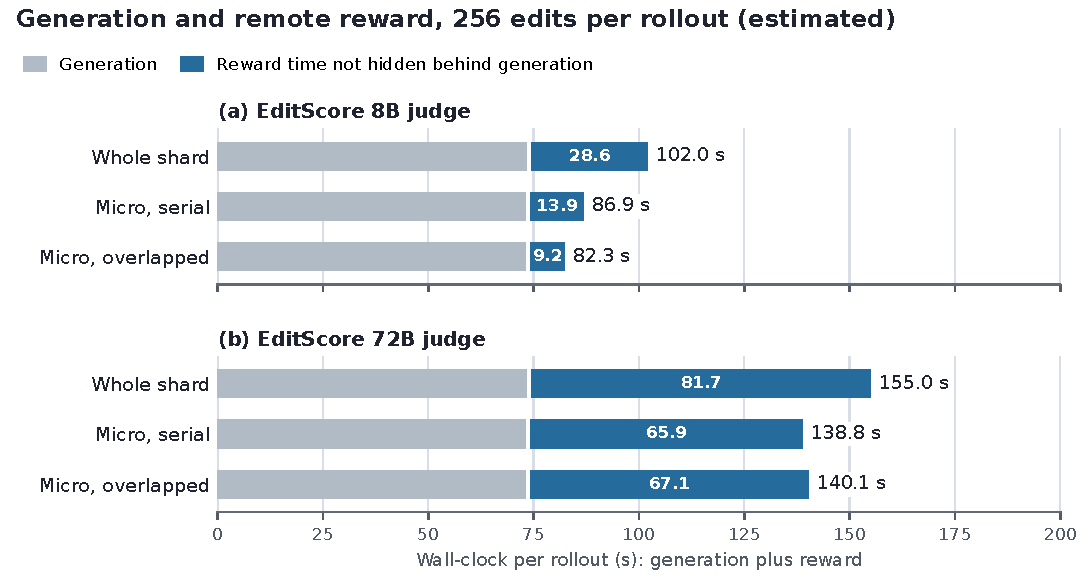
\includegraphics[width=0.85\textwidth]{artifacts/reported_results/2026-09-30-reward-service/figures/overlap_wallclock.pdf}
\caption{Breakdown of rollout wall-clock time for the two remote EditScore judges in Table~\ref{tab:reward-overlap} (estimated as described in the table caption). Generation duration is constant across schedules; the schedules differ in the portion of reward evaluation time exposed outside generation.}
\label{fig:reward-overlap}
\end{figure}

\paragraph{Batch-size overhead of micro-batched requests.}
Splitting a shard into smaller requests increases total judge compute time when the server does not batch across concurrent requests.
On the 72B judge, an eight-pair request requires \RSLargeSerialService{}\,s whereas a 32-pair request requires \RSLargeWholeService{}\,s, increasing total judge work per rollout from \RSLargeWholeWork{}\,s (whole shard) to \RSLargeSerialWork{}\,s (micro-batched); on the 8B judge, the corresponding totals are \RSSmallWholeWork{}\,s and \RSSmallMicroWork{}\,s (with per-pair costs of \RSLargeMicroPerPair{}\,s versus \RSLargeWholePerPair{}\,s on 72B and \RSSmallMicroPerPair{}\,s versus \RSSmallWholePerPair{}\,s on 8B).
Micro-batched scheduling reduces wall-clock time despite this overhead because judge evaluation begins one quarter of the way through generation rather than after all generation completes.
When requests are split into smaller chunks \emph{without} interleaving them with generation, only the batch-size penalty remains: in an ablation at 16 rows per rank, splitting the post-generation whole-shard call into two eight-row requests increased total time from \RSSmallShallowBase{}\,s to \RSSmallShallowSplit{}\,s on the 8B judge and from \RSLargeShallowBase{}\,s to \RSLargeShallowSplit{}\,s on the 72B judge.
Adding cross-request continuous batching or additional judge replicas would eliminate the small-batch penalty while preserving the early-start advantage of micro-batching.

\paragraph{In-process scoring baseline.}
When PickScore runs in-process on the policy workers, reward evaluation accounts for roughly 1\,s of compute per rollout, and \texttt{RewardStack} reduces combined generation and reward time from \RSLocalBase{}\,s to \RSLocalSerial{}\,s primarily by eliminating the separate driver-level dispatch hop.
Because in-process scoring is already negligible relative to generation, background thread overlap provides no additional reduction (\RSLocalSerial{}\,s versus 52.3\,s).

\paragraph{Interaction with training-phase memory collection.}
Executing multiple generation and scoring micro-batches within a single rollout leaves uncollected Python objects and cached allocations in the worker heap.
When the subsequent training phase began without an explicit garbage-collection and cache-flush pass at the rollout boundary, training step time increased from \RSTrainRemoteCollect{}\,s to \RSTrainRemoteNoCollect{}\,s in the 8B-judge runs and from \RSTrainLocalCollect{}\,s to \RSTrainLocalNoCollect{}\,s in the in-process PickScore runs.
The merged \texttt{RewardStack} implementation therefore triggers a cleanup pass once the scored shard leaves the worker.
Because the training phase replays against the trainer's own conditioning in both configurations, these training durations are direct measurements rather than rescaled estimates, illustrating why rollout scheduling changes must be evaluated across the full iteration.

\subsection{GPU Sharing Across Lightweight Scorers via MPS}
\label{sec:reward-mps}

By default, the standalone reward service allocates whole GPUs to each scorer actor.
While this provides hardware fault isolation, a panel of lightweight preference models leaves a high-memory accelerator largely underutilized.
Although Ray supports fractional GPU allocation to colocate multiple actors on a single device, standard CUDA contexts from separate processes are time-sliced by the driver.
NVIDIA Multi-Process Service (MPS) allows kernels from distinct processes to execute concurrently on the same GPU~\citep{nvidiamps}, preserving per-scorer process and dependency isolation while overlapping their compute kernels.

UniRL pull request~\#492 introduces an opt-in MPS runtime mode for the standalone reward service.
The service can either manage the node's MPS control daemon directly---starting it before any scorer actor initializes CUDA and stopping it after all actors exit---or attach to an externally managed daemon.
Each scorer configuration may specify an active-thread percentage and a device-memory allocation cap, which are exported to the actor's environment prior to CUDA initialization.
Startup validation rejects MPS configurations that combine device sharing with tensor-parallel scorers, unqualified scorer backends, or half-precision weights running below a 100\% active-thread cap.
During shutdown, the service halts request admission, drains in-flight GPU work, and terminates actors before stopping the MPS daemon.
Because the MPS memory cap bounds per-client allocations without providing hardware memory protection, all actors sharing a GPU belong to a single fault domain, which is recorded in the service's health metadata.

\begin{table}[H]
\caption{Throughput gain (\%) of NVIDIA MPS over fractional GPU colocation without MPS for two or three replicas of a single scorer on one NVIDIA H20 GPU, as reported in UniRL pull request~\#492; $B_s$ denotes the scorer batch size. Dashes indicate batch sizes at which the scorer implementation does not execute a single batched forward pass.}
\label{tab:reward-mps}
\centering
\small
% Generated by artifacts/reported_results/2026-09-30-reward-service/generate.py; do not edit.
\begin{tabular}{@{}lrrrrrr@{}}
\toprule
 & \multicolumn{3}{c}{Two copies} & \multicolumn{3}{c}{Three copies} \\
\cmidrule(lr){2-4}\cmidrule(l){5-7}
Scorer & $B_s{=}1$ & $B_s{=}4$ & $B_s{=}8$ & $B_s{=}1$ & $B_s{=}4$ & $B_s{=}8$ \\
\midrule
CLIP & $+$11.2 & $+$20.0 & $+$14.8 & $+$16.5 & $+$24.4 & $+$19.2 \\
HPSv2 & $+$17.4 & -- & -- & $+$48.4 & -- & -- \\
ImageReward & $+$24.0 & -- & -- & $+$40.8 & -- & -- \\
HPSv3 & $+$20.6 & $+$11.2 & -- & $+$22.6 & $+$12.8 & -- \\
GOT-OCR & $-$2.8 & -- & -- & $-$3.2 & -- & -- \\
\bottomrule
\end{tabular}

\end{table}

\paragraph{Reported qualification results.}
Table~\ref{tab:reward-mps} summarizes the qualification benchmarks reported in UniRL pull request~\#492 on NVIDIA H20 GPUs (these measurements were not independently rerun for this report).
For heterogeneous panels colocated on a single H20 GPU, the pull request reports a median throughput gain of \RSMpsThreeLight{} for three lightweight scorers and \RSMpsTwoLight{} for two, smaller gains when a heavier vision--language scorer dominates device time, and no gain for an autoregressive OCR scorer.
On the deterministic test fixture, output scores were bit-identical with and without MPS enabled.
Profiling in the pull request indicates that a single CLIP replica at $B_s{=}1$ utilizes roughly half of the device's execution time, allowing MPS to fill the inter-kernel gaps with work from colocated replicas; once a single scorer saturates the GPU, MPS provides no additional throughput.

\paragraph{Numerical correctness boundary.}
The same qualification identified a numerical defect on the tested H20 driver stack when restricting the MPS active-thread percentage below 100\%: half-precision matrix multiplications produced non-finite outputs in CLIP and finite but numerically incorrect values in PickScore.
Consequently, the runtime rejects half-precision scorers configured with less than a 100\% active-thread share.
A separate review on a different GPU model and driver version did not reproduce the numerical corruption and observed negligible colocation overhead even without MPS because the workload was bottlenecked by CPU preprocessing and HTTP serialization.
Both the throughput benefit and the sub-100\% thread-cap hazard are therefore hardware- and driver-dependent.
Only CLIP and PickScore at a 100\% active-thread share are marked qualified in UniRL pull request~\#492; vision--language judges, long-horizon stability runs, and sharing GPUs between reward actors and policy workers remain outside its qualified scope.
